\documentclass{sig-alternate-ipsn13}
\usepackage{amsmath,graphicx,pifont}

\begin{document}

\title{Project Report: Finite Elements Analysis for OsteoApp}

\numberofauthors{3}

\author{
  \alignauthor
  Baihan Lin\\
         \affaddr{UbiComp Lab}\\
         \affaddr{University of Washington} \\
         \email{doerlbh@gmail.com}
}

\date{10 February 2017}

\maketitle

%----------------------------------------%
%-----------------ABSTRACT---------------%
%----------------------------------------%

\begin{abstract}
The project aims to conduct a finite element analysis (FEA) on a bone-like structure to simulate the vibration properties of a bone or arm. This simulation is supportive to OsteoApp, a smartphone app for personal osteoporosis screening that tests bone density and tells people if they are at risk for bone disease. OsteoApp uses a vibration technique that takes advantage of the accelerometers on a hand-held smartphone to measure bone stiffness and density, based on the vibrations that pass through the user’s arm when the elbow is tapped. The FEA simulation in this study can help us better understand the relationship between the external tapping with the measured signals. This study is conducted by Baihan Lin, mentored by Morelle Arian and Josh Fromm, and supervised by Prof. Shwetak Patel.
\end{abstract}

%----------------------------------------%
%---------------INTRODUCTION-------------%
%----------------------------------------%

\section{Project Description} 

The finite element analysis (FEA) on a bone-like structure to simulate the vibration properties of a bone or arm. This simulation is supportive to OsteoApp, a smartphone app for personal osteoporosis screening that tests bone density and tells people if they are at risk for bone disease. OsteoApp uses a vibration technique that takes advantage of the accelerometers on a hand-held smartphone to measure bone stiffness and density, based on the vibrations that pass through the user’s arm when the elbow is tapped. The FEA simulation in this study can help us better understand the relationship between the external tapping with the measured signals. 

You will need to have a clear idea for what you are making, why you are making it, and where it fits in with the current state of the art. In the project description section cover:

\begin{itemize}
\item What is the purpose of your device? Who will use the system. What are the challenges in developing the device. This is a good time for coherent rambling and brainstorming.
\item Talk about the current state of your development area. What has been done similarly, what will you be doing better. How will you utilize the power of BLE and the sensors to advance the state of the art.
\item Talk about the current state of your development area. What has been done similarly, what will you be doing better. How will you utilize the power of BLE and the sensors to advance the state of the art.
\end{itemize}

This section needs to be two paragraphs at minimum. Search google scholar while on campus (all papers are free) and see if you can find related work.

%----------------------------------------%
%----------------SENSORS-----------------%
%----------------------------------------%

\section{Progress} 

Currently, I have constructed a 

\subsection{2017/03/30: Interview, Setup}


\subsection{2017/04/04: Decide on project}


\subsection{2017/04/11: Basic construction of model}

\begin{figure}
  \centering 
	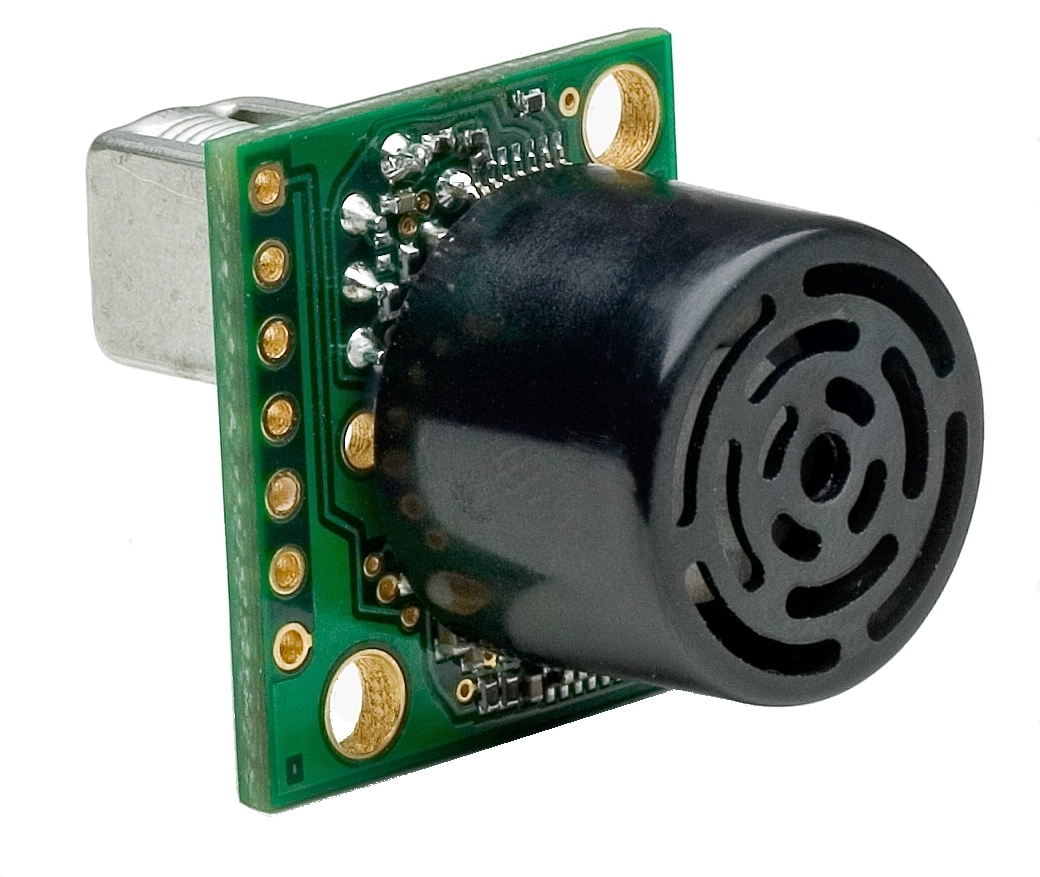
\includegraphics[width=2in]{images/sensor.jpg}
    \caption{Memeographer sensor}
    \label{fig:Memeographer}
\end{figure}

\subsection{Sensor 3: Rhombascope}

Include part number, price, if relevant an image. Each sensor needs to be thoroughly discussed in terms of how it fits in and why you chose it.

%----------------------------------------%
%--------------SYSTEM-DESIGN-------------%
%----------------------------------------%

\section{System Design} 

Here you will do all of your back of the envelope calculations for power, decide on communication protocols, and make educated size predictions. 

\subsection{Power Analysis}

Include a power systems diagram like in the presentations. A sample table is added below. You should be adding and removing columns as needed depending on your needs to summarize the power requirements of each sensor.

\begin{center}
\begin{tabular}{|c|c|c|}
\hline
 Sensor & $I_{min}$ & $V_{min}$ \\ 
 \hline
 Awesomiter & 100mA & 4.7V \\  
 Memographer & 3mA & 2.0V \\
 Rhombascope & 7A & 3.3V \\
 \hline
\end{tabular}
\end{center}

Add a paragraph talking about expected usage and how that relates to your power consumption and battery size. Put derivations for ALL calculations here as equations:

\begin{equation}
V = IR
\end{equation}

Latex is a standard for publications, you can google how to write equations and symbols such as $\alpha,\beta$ etc. 

\subsection{Communications}

\begin{figure}
  \centering 
	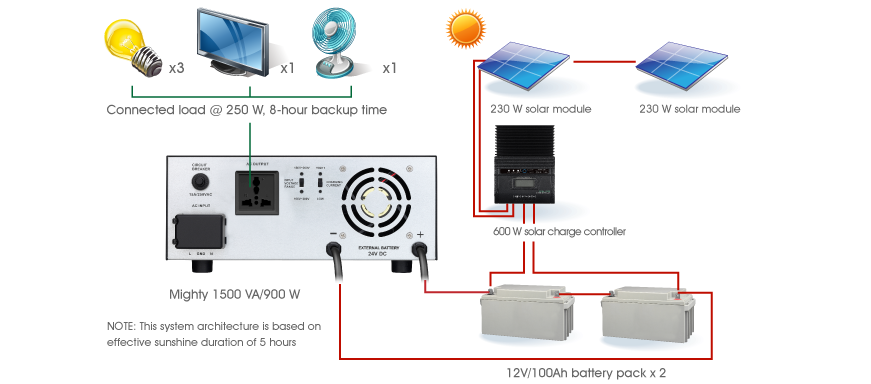
\includegraphics[width=\columnwidth]{images/power.png}
    \caption{Power Diagram}
    \label{fig:PowerDiagram}
\end{figure}

Insert a communications diagram like in the presentations and figure \ref{fig:PowerDiagram}. Add a discussion on what sampling frequencies each sensor will be using and relate it to your overall system analysis for power consumption etc. Talk about sleep cycling and how your sampling affects it.

\subsection{Enclosure Design}

Create a 3D model of your device along with dimensions. This time around you should have selected your sensors and battery based on well thought out power requirement calculations. The 3D render should include all large components. Sensors that are not SMD should be included. Things like the PSoC chip and resistors are not necessary but larger things are. Battery is a must based on dimensions from vendor. Add dimension markers in render. Remember you will be 3D printing your enclosure so the sky is the limit.

\begin{figure}
  \centering 
	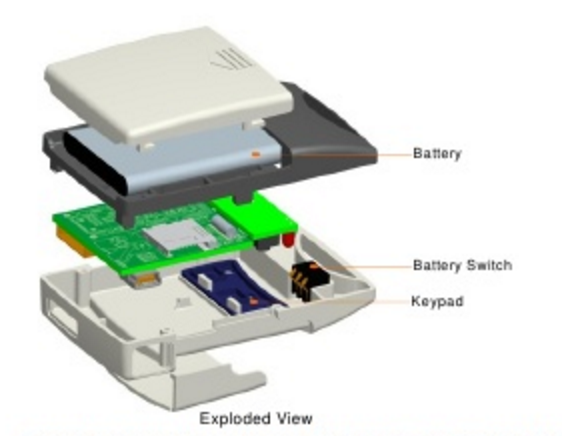
\includegraphics[width=\columnwidth]{images/enclosure.png}
    \caption{Enclosure and Internals}
    \label{fig:Enclosure}
\end{figure}

%----------------------------------------%
%-------------DEVICE-FIRMWARE------------%
%----------------------------------------%

\section{Device Firmware} 
\label{sec:Firmware}

Here you will put your PSoC firmware deliverables.

\subsection{System Diagram}

This is a general flow chart of how your system will work. It is meant to be a nice overview of how everything connects on a high level. The diagram will probably be wide so I put an example of how to put a two column image in your document using latex. Check out figure \ref{fig:SystemOverview}. There is no correct or wrong way to do this system diagram. 

\begin{figure*}[h!]
  \centering 
	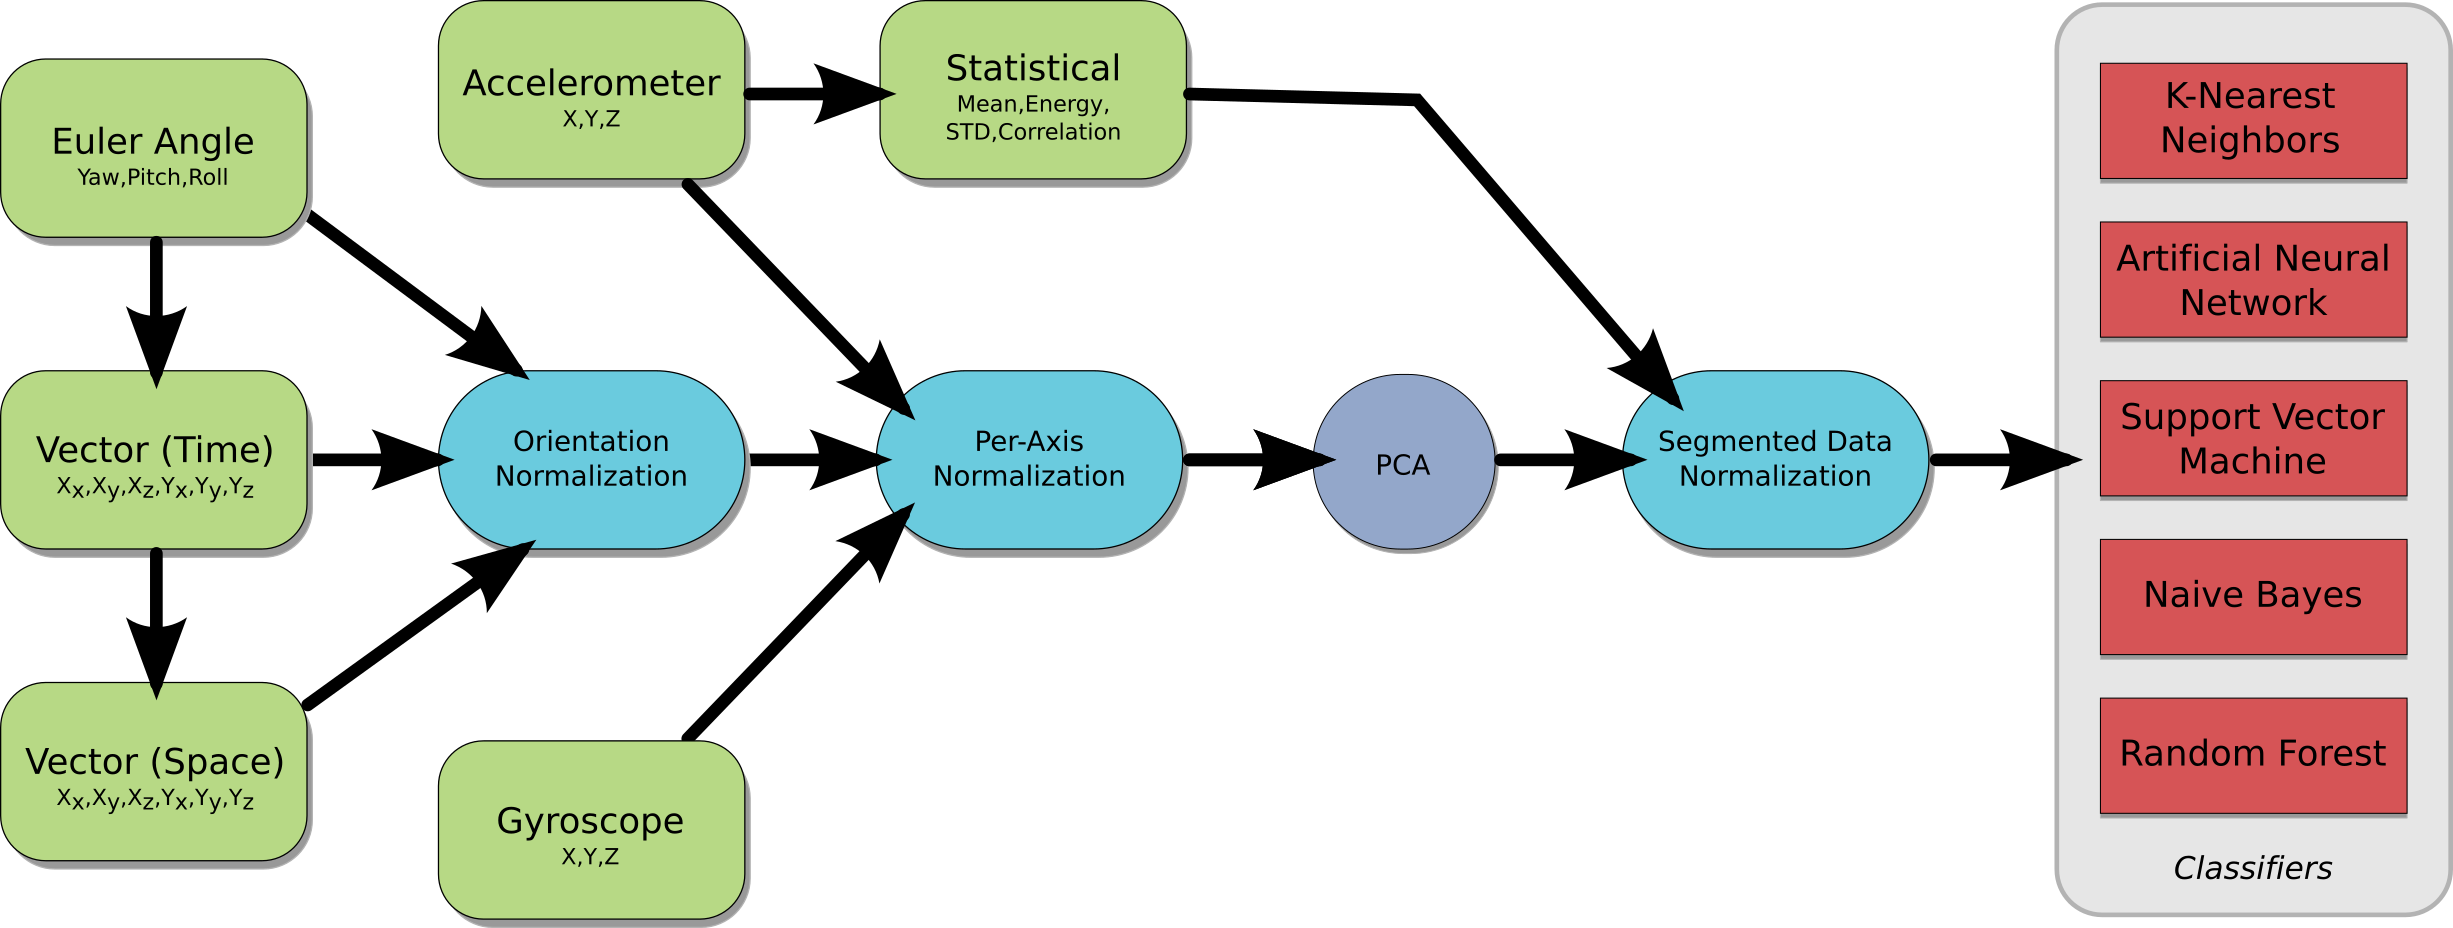
\includegraphics[width=5.6in]{images/top.png}    
    \caption{System Overview}
    \label{fig:SystemOverview}
\end{figure*}

\subsection{Signals Chart}

You need a signals chart like in \ref{fig:Signals}. Again, this was done in the presentations so should not come as a surprise.

\begin{figure}
  \centering 
	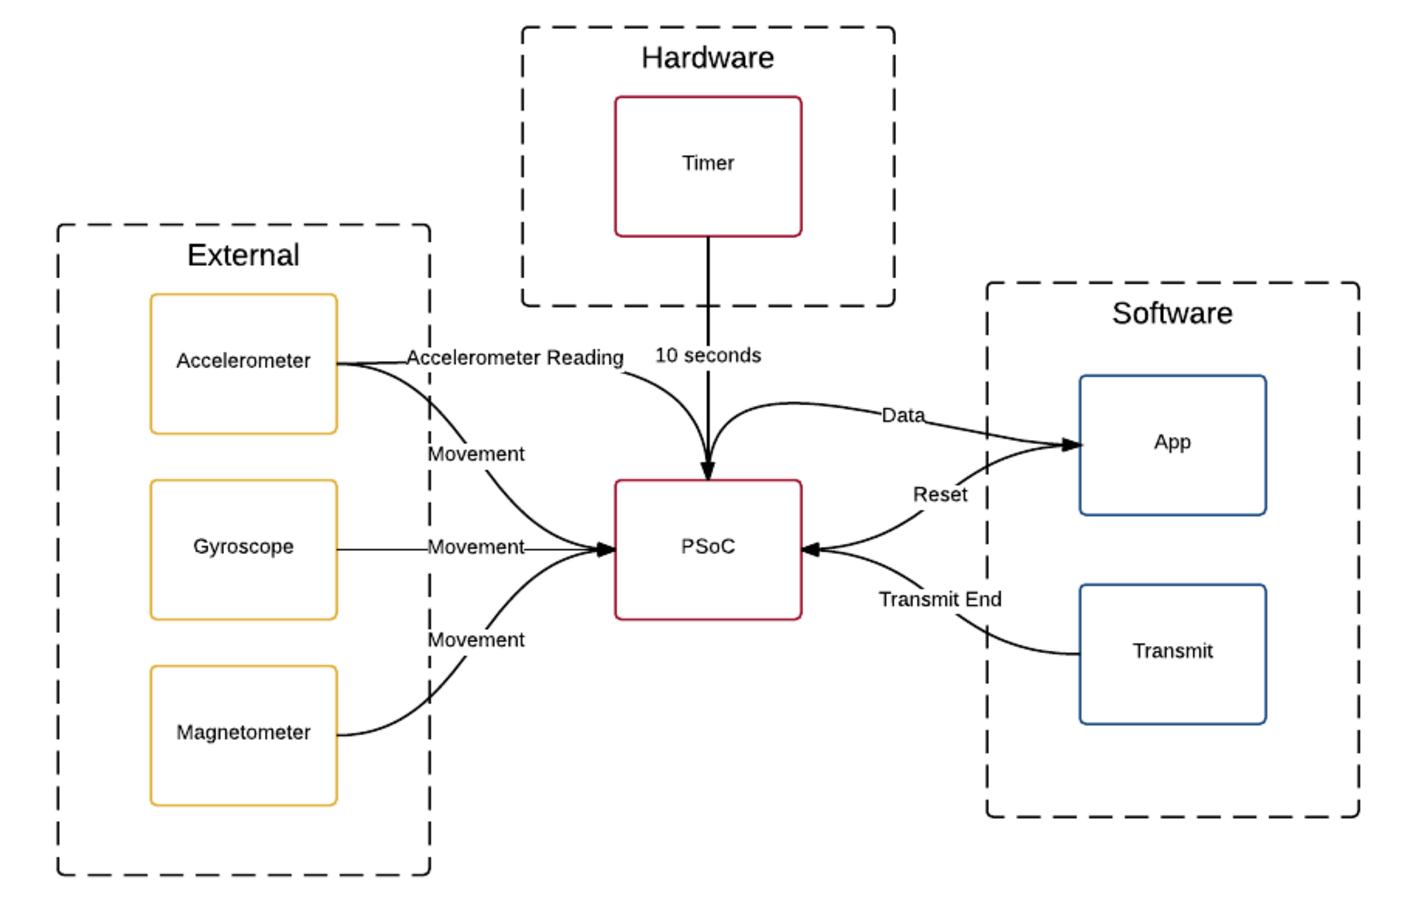
\includegraphics[width=\columnwidth]{images/signals.png}
    \caption{Signals Chart}
    \label{fig:Signals}
\end{figure}

\subsection{State Machine}

And you will also need a well designed state machine following the convention put forth over the past two presentations. 

%----------------------------------------%
%-----------MOBILE-APPLICATION-----------%
%----------------------------------------%

\section{Mobile Application} 

Same as the presentation; add screenshots of a preliminary application. Include a list of features that will be available at the end of the quarter and two case studies outlining how a typical usage of your device will look like. Each of the two case studies should describe a particular scenario in which the app would be used together with the device to achieve something useful. For example:  \textit{Bob frequently loses his keys. Bob is smart and bought a Tile device to attach to his keys. Now, whenever Bob loses his keys, he uses the smartphone app to blink an LED on the Tile device, vibrate the device, and generate a chirping sound so Bob can locate his keys. Bob does not lose his keys anymore. Be like Bob, buy a Tile.}

%----------------------------------------%
%-------------PROJECT-BUDGET-------------%
%----------------------------------------%

\section{Project Budget} 

Here you should do a detailed cost analysis including pie charts for the cost breakdown for the bill of materials (BOM) per device or system. Check out Figure \ref{fig:Cost} for an example pie chart. The component costs should be calculated for two different scales of production, resulting in two different pie charts; one for an individual order and one for a bulk order (e.g., 1,000 devices). Also produce a table that shows cost estimates (broken down into different categories) for the entire quarter, resulting in the summed total for the quarterly cost estimate for the project. The non-recurring engineering (NRE) cost should be included in the quarterly cost estimates table, but it should not be part of the pie charts, since the NRE cost is not dependent upon the number of devices sold. For the NRE cost, choose a reasonable salary to pay yourselves as though you were working in a startup company. You can use your Gantt chart timeline to estimate the amount of time spent developing the product, and thus the amount of money you will need to pay each member of the team.

\begin{figure}
  \centering 
	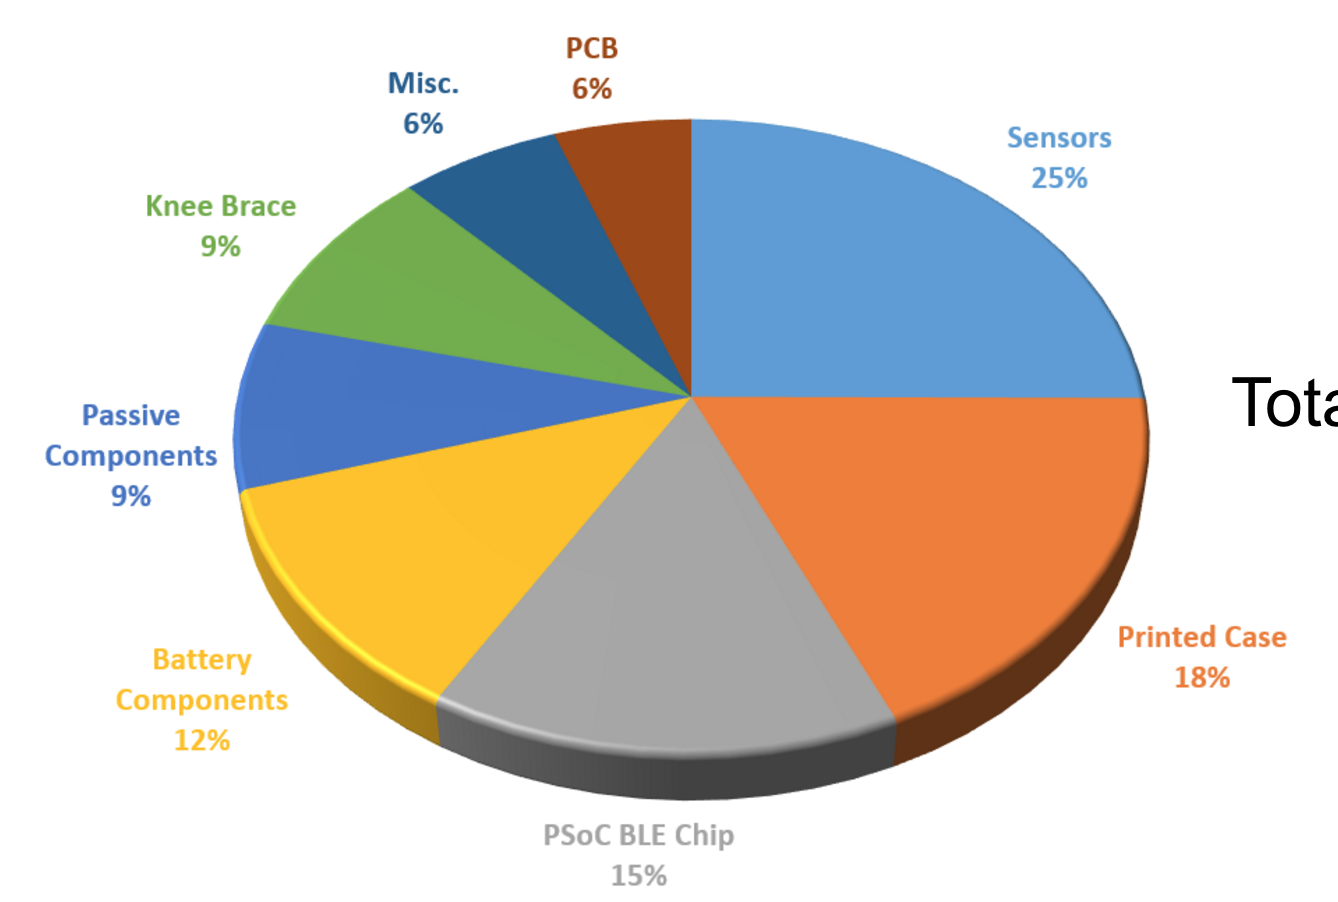
\includegraphics[width=\columnwidth]{images/cost.png}
    \caption{Cost Diagram}
    \label{fig:Cost}
\end{figure}

%----------------------------------------%
%---------------CONCLUSION---------------%
%----------------------------------------%

\section{Conclusion} 

Briefly review the most important points from your report to reinforce them and provide a takeaway message for the reader of the report. 

%----------------------------------------%
%---------------BIBLIOGRAPHY-------------%
%----------------------------------------%

%\bibliographystyle{abbrv}
%\bibliography{sigproc}  

\end{document}